\usetikzlibrary{arrows.meta,calc,circuits.logic.US,decorations.pathreplacing,matrix,positioning}

\begin{frame}[fragile,label=truthTables]{interlude: a truth table}
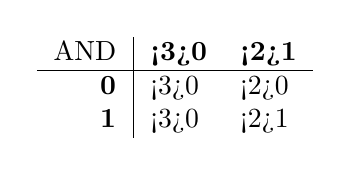
\begin{tikzpicture}
\node (and) {
\begin{tabular}{r|ll}
    AND & \bf \myemph<3>{0} & \bf \myemph<2>{1} \\ \hline
    \bf0 & \myemph<3>{0} & \myemph<2>{0} \\
    \bf1 & \myemph<3>{0} & \myemph<2>{1} \\
\end{tabular}
};
\end{tikzpicture}
    \begin{itemize}
        \item<2-> \myemph<2>{AND with 1}: keep a bit the same
        \item<3-> \myemph<3>{AND with 0}: clear a bit
        \vspace{.5cm}
        \item<4-> method: construct ``mask'' of what to keep/remove
    \end{itemize}
\end{frame}

\begin{frame}[fragile,label=bitwiseAnd]{bitwise AND --- {\tt \&}}
\begin{columns}[b]
\begin{column}{0.6\textwidth}
\lstset{
    moredelim=**[is][\btHL<1>]{@1*}{*@},
    moredelim=**[is][\btHL<2>]{@2*}{*@},
    moredelim=**[is][\btHL<3>]{@3*}{*@},
    moredelim=**[is][\btHL<4>]{@4*}{*@},
    moredelim=**[is][\btHL<5>]{@5*}{*@},
    moredelim=**[is][\btHL<6>]{@6*}{*@},
    escapechar=$,
}
\begin{itemize}
\item Treat value as \myemph{array of bits}
\item \lstinline|1 & 1 == 1|
\item \lstinline|1 & 0 == 0|
\item \lstinline|0 & 0 == 0|
\item \lstinline|@2*2 & 4 == 0*@|
\item \lstinline|@3*10 & 7 ==  2*@|
\end{itemize}
\vspace{0pt}
\end{column}
\begin{column}{0.4\textwidth}
\onslide<2->{
\tt
\begin{tabular}{llllll}
~  & \ldots & 0 & 0 & 1 & 0 \\
\&\hspace{.5cm} & \ldots & 0 & 1 & 0 & 0 \\\hline
~  & \ldots & 0 & 0 & 0 & 0
\end{tabular}
}
\vspace{1cm}
\onslide<3->{
\tt
\begin{tabular}{llllll}
~  & \ldots & 1 & 0 & 1 & 0 \\
\&\hspace{.5cm} & \ldots & 0 & 1 & 1 & 1 \\\hline
~  & \ldots & 0 & 0 & 1 & 0
\end{tabular}
}
\vspace{0pt}
\end{column}
\end{columns}
\end{frame}

\begin{frame}[fragile,label=bitwiseAndCAsm]{bitwise AND --- C/assembly}
    \begin{itemize}
    \item x86: {\tt {\keywordstyle and} \%reg, \%reg}
    \item C: \verb|foo & bar|
    \end{itemize}
\end{frame}

\begin{frame}[fragile,label=bitwiseHW]{bitwise hardware ({\tt10 \& 7 == 2})}
\begin{tikzpicture}[circuit logic US]
\node (num1) {\tt 10};
\coordinate (num1Intersect) at ($(num1) + (0, -1cm)$);
\draw[very thick] (num1) -- (num1Intersect);
\node[right=9cm of num1] (num2) {\tt 7};
\coordinate (num2Intersect) at ($(num2) + (0, -2cm)$);
\draw[very thick] (num2) -- (num2Intersect);

\matrix(ands) [
    below=2cm of num1,
    xshift=-.36cm,
    anchor=north west,
    matrix of nodes,
    column sep=.5cm,
    nodes={
        draw,
        fill=black!5,
        and gate,
        point down,
        logic gate inputs=nn
    }] {
    ~ \& |[draw=none,fill=none,rectangle]| \vdots \& ~ \& ~ \& ~ \& ~ \& ~ \& ~ \& ~ \\
};
\foreach \x in {1,3,4,5,6,7,8,9} {
    \draw[thin] ($(num1Intersect)-(0.4pt,0)+(0.\x pt,0)$) -- ($(num1Intersect) + (0mm,-2mm) + 3*(0.\x mm,0.\x mm)$) -| (ands-1-\x.input 2);
    \draw[thin] ($(num2Intersect)-(0.4pt,0)+(0.\x pt,0)$) -- ($(num2Intersect) + (0mm,-2mm) + 3*(-0.\x mm,0.\x mm)$) -| (ands-1-\x.input 1);
}
\begin{scope}[every node/.style={yshift=-1.2mm,font=\small\tt,xshift=1mm}]
\node[above left=0pt of ands-1-9.input 2] {0};
\node[above left=0pt of ands-1-8.input 2] {1};
\node[above left=0pt of ands-1-7.input 2] {0};
\node[above left=0pt of ands-1-6.input 2] {1};
\node[above right=0pt of ands-1-9.input 2] {1};
\node[above right=0pt of ands-1-8.input 2] {1};
\node[above right=0pt of ands-1-7.input 2] {1};
\node[above right=0pt of ands-1-6.input 2] {0};
\end{scope}
\begin{scope}[every node/.style={font=\small\tt}]
\node[below=1cm of ands-1-9.output] (res9) {0};
\node[below=1cm of ands-1-8.output] (res8) {1};
\node[below=1cm of ands-1-7.output] (res7) {0};
\node[below=1cm of ands-1-6.output] (res6) {0};
\end{scope}
\foreach \x in {1,3,4,5} {
    \coordinate (res\x) at ($(ands-1-\x.output) + (0,-1cm)$);
}
\foreach \x in {1,3,4,5,6,7,8,9} {
    \draw[thin] (ands-1-\x.output) -- (res\x);
}

\end{tikzpicture}
\end{frame}

